\documentclass{article}

% Packages
\usepackage{fancyhdr}
\usepackage{setspace}
\usepackage{titlesec}
\usepackage{tocloft}
\usepackage{lipsum} % For placeholder text
\usepackage[fleqn]{amsmath}
\usepackage{amssymb}
\usepackage{hyperref}
\usepackage{url}
\usepackage{graphicx}
\usepackage{geometry}
\usepackage{babel}
\usepackage{enumitem}
\usepackage{parskip}
\usepackage{chemfig}
\usepackage{pdfpages}
\usepackage{tikz}
\usepackage{fancybox}
\usepackage{makecell}
\usepackage{pgfplots}
\usepackage{soul}
\usepackage{ulem}
\usepackage{wrapfig}
\usepackage{subcaption}
\usepackage[T1]{fontenc}
\usepackage{esvect}
\usepackage{xcolor}
\usetikzlibrary{arrows}
\usetikzlibrary{decorations.pathreplacing}
\pgfplotsset{compat=1.17}

\geometry{
    a4paper,
    total={170mm, 257mm},
    left=20mm,
    top=20mm
}

\hypersetup{
    colorlinks=true,
    linkcolor=black,
    urlcolor=blue,
    pdftitle={Context 1}
}

\pagestyle{fancy}
\fancyhf{}
\fancyhead[L]{\leftmark}
\fancyhead[R]{\thepage}
\renewcommand{\headrulewidth}{0.4pt}

\titleformat{\chapter}[block]{\bfseries\LARGE}{\thechapter.}{1em}{}

\begin{document}

\begin{titlepage}
    \begin{center}
        \vspace*{2cm}
        
        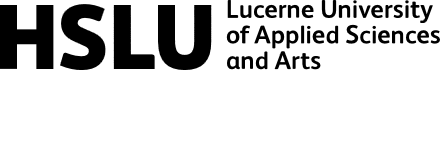
\includegraphics[width=0.5\textwidth]{media/hslu-svg-logo.png} % Replace 'company_logo.png' with your logo file
        
        \vspace{1.5cm}
        
        {\Huge \textbf{Project Documentation}}
        
        \vspace{0.5cm}
        
        {\LARGE Research on My$_{\text{celium}}$Tent and Wotagarden}
        
        \vspace{2cm}
        
        {\large \textbf{Team Members:}}
        
        \vspace{0.5cm}
        
        {\Large
            Althaus Simon \\
            Berner Nic \\
            Frongillo Matteo \\
            McCarthy Benjamin \\
            Nyamdorj Narandavaa
        }
        
        \vfill
        
        {\large
            Company Name \\
            Department Name \\
            \today
        }
        
    \end{center}
\end{titlepage}

\tableofcontents
\thispagestyle{empty}
\newpage

\chapter{Introduction}

\chapter{MyceliumTent Research}

\chapter{Wotagarden Research}

\chapter{Meeting Report}

\section{Planned Agenda Items}
\begin{itemize}
    \item Selection of project ideas
    \item Organizational chart and distribution of roles
    \item Project plan
    \item Next steps
    \item Open questions
\end{itemize}

\section{Discussed, Feedback, Decisions}

\subsection{Selection of Project Ideas}
“Wotagarden” presents a new construction area on water. It can be used by private, as well as public users for many different purposes, e.g., sunbathing.

“MyceliumTent” is a solution for a part of the big amounts of waste produced at festivals. It is a product made from mushroom powder, used by young festival-goers and campers seeking a cheap, easy-to-use, and sustainable place to sleep.

\subsection{Organizational Chart and Distribution of Roles}
The organizational chart and included tasks for each role were explained.

\subsection{Project Plan}
The format and functionality of the project plan were briefly described.

\subsection{Next Steps}
The next steps and the allocation of the roles should be discussed in the team and are not a part of the review meeting.

\subsection{Questions}
Question about the professional background of each member of the team.

\subsection{Feedback}
\begin{itemize}
    \item All of the team members present well and confidently.
    \item The project plan is well constructed.
    \item Feedback for the Review 1 Document will be sent to our team by Anna Christen after the meeting.
    \item The invitation to the meeting should only be sent via email, not Microsoft Teams.
\end{itemize}

\subsection{Decisions}
Christen Anna and Rohrer Julia both agree that the “MyceliumTent” should be pursued.

\section{Agenda Items for Next Meeting}
\begin{itemize}
    \item Final user scenario
    \item Feedback to potential customers
    \item Requirement specifications
\end{itemize}

\vspace{1cm}
\noindent\textit{Written by: Matteo Frongillo}

\chapter{References}
% \bibliographystyle{plain}
% \bibliography{references} % Uncomment and replace 'references' with your .bib file if needed

\end{document}